\documentstyle[11pt,epsfig,fancybox,semcolor,semlayer,doublespace,portrait]
{seminar}
\input clp_utils

% The following strings are needed by the title page and 
% page style definitions in map_utils.tex
\newcommand{\talktitle}[0]{Two Kalman Bugs Fixed}
\newcommand{\fmttitle}[0]{}
\newcommand{\conftitle}[0]{CLEO Plenary}
\newcommand{\myname}[0]{Jim Pivarski}
\newcommand{\affila}[0]{Cornell University}
\newcommand{\talkdate}[0]{January 25, 2003}

\pagestyle{conference}   % From clp_utils.tex

% slide magnification
\slidesmag 1

%%%%%%%%%%%%%%%%%%%%%%%%%%%%%%%%%%%%%%%%%%%%%%%%%%%%%%%%%%%%%%%%%%%%%%%%%%%
% Start document
\begin{document}

% Set page size
\slideheight 7.0in
\slidewidth 8.8in 

% Set array stretch
\renewcommand{\arraystretch}{0.3}
\renewcommand{\slidetopmargin}{0.4in}
\renewcommand{\slidebottommargin}{0.9in}


%%%%%%%%%%%%%%%%%%%%%%%%%%%%%%%%%%%%%%%%%%%%%%%%%%%%%%%%%%%%%%%%%%%%%%%%%%%

\begin{slide*}

\slideframe{}
\slideframe*[\dkblue]{Oval}

\begin{center}
\vspace{4 cm}
{\Huge Two Kalman Bugs Fixed}  \\
\vspace{1 cm}
{\LARGE	Jim Pivarski } \\
\vspace{2 cm}
\conftitle \\
{\large \talkdate}

\end{center}

\end{slide*}

% %%%%%%%%%%%%%%%%%%%%%%%%%%%%%%%%%%%%%%%%%%%%%%%%%%%%%%%%%%%%%%%%%%%%%%%%%%%

\begin{slide*}

\slideframe{}
\slideframe*[\dkblue]{Oval}
\huge
\heading{Two Kalman Bugs}
\Large

\begin{minipage}[t]{\linewidth}

\vspace{1cm}

\begin{tabular}{r l}
{\bf MissingBeamWall} & \begin{minipage}[t]{0.57\linewidth}
Beamwall scattering not applied on the negative-z half of the
beampipe. \\
\begin{center}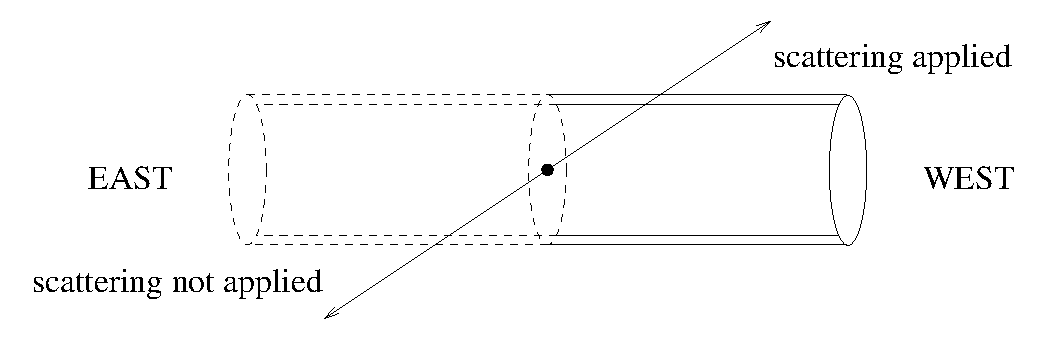
\includegraphics[width=0.8\linewidth]{bug_MissingBeamWall.eps}\end{center}
\begin{itemize}
  \item Negligible effect on track parameters
  \item 0\% -- 20\% effect on error matrix
    \mbox{elements}
\end{itemize}
\end{minipage} \\

\vspace{1cm} \\

{\bf BigErrorMatrix} & \begin{minipage}[t]{0.57\linewidth}
When beamwall scattering was not applied, some outward fits have large
error matrices.
\begin{itemize}
  \item 10\% of outward fits were affected
  \item Most affected tracks have no RICH information
\end{itemize}
\end{minipage} \\

\end{tabular}

\end{minipage}

\end{slide*}

% %%%%%%%%%%%%%%%%%%%%%%%%%%%%%%%%%%%%%%%%%%%%%%%%%%%%%%%%%%%%%%%%%%%%%%%%%%%

\begin{slide*}

\slideframe{}
\slideframe*[\dkblue]{Oval}
\huge
\heading{MissingBeamWall Bug}
\Large

\begin{minipage}[t]{\linewidth}

\vspace{0.5cm}

{\huge \bf How did this happen?}

To work around an artificial limitation in GEANT, the IR geometry
description was replaced by a description of the west side only, then
replicated on the east side by mirror symmetry.

\vspace{0.1cm}
\begin{center}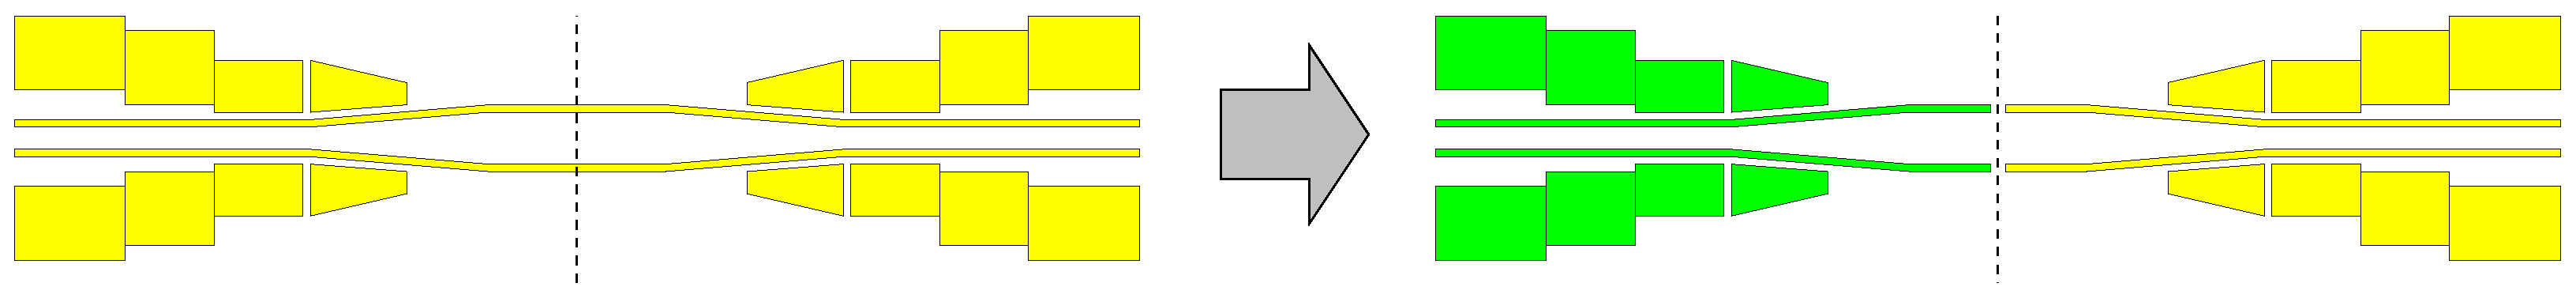
\includegraphics[width=\linewidth]{change_IRGeom.eps}\end{center}
\vspace{0.1cm}

Kalman only looked for the first instance of beamwall objects.

\vspace{0.1cm}
\begin{center}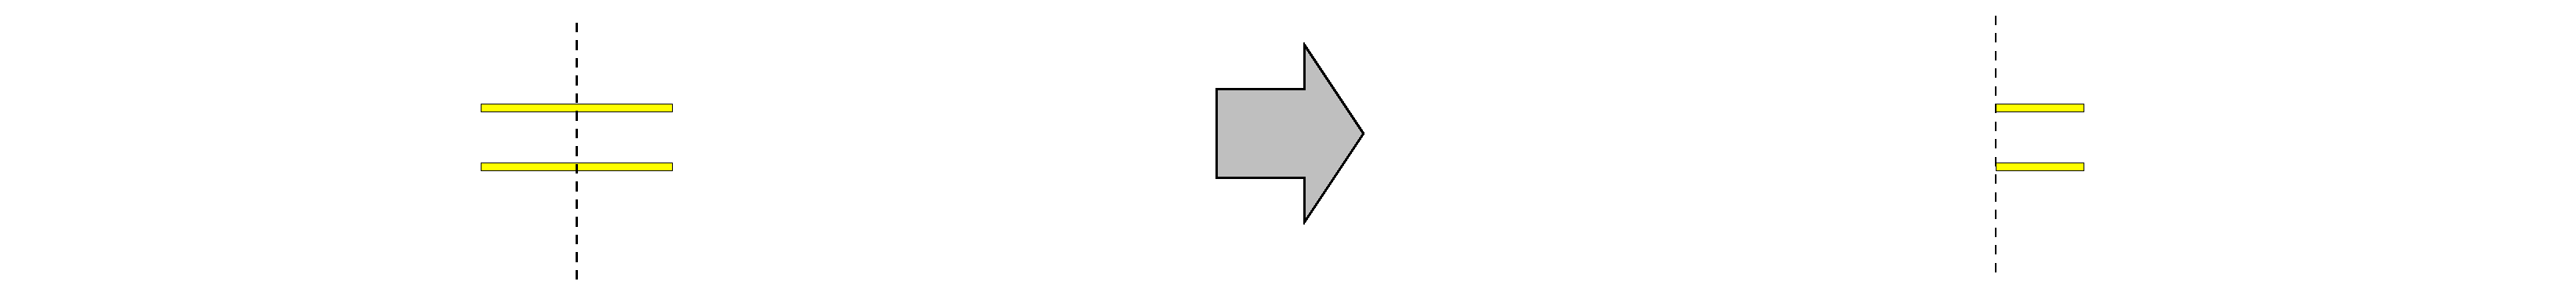
\includegraphics[width=\linewidth]{change_IRGeom2.eps}\end{center}

\vspace{0.5cm}

{\huge \bf What is the scale of the error?}

\begin{center}\includegraphics[width=\linewidth]{howbig2.eps}\end{center}

\end{minipage}

\end{slide*}

% %%%%%%%%%%%%%%%%%%%%%%%%%%%%%%%%%%%%%%%%%%%%%%%%%%%%%%%%%%%%%%%%%%%%%%%%%%%

\begin{slide*}

\slideframe{}
\slideframe*[\dkblue]{Oval}
\huge
\heading{BigErrorMatrix Bug}
\Large

\begin{minipage}[t]{\linewidth}

\vspace{0.5cm}

{\huge \bf How did this happen?}

\vspace{-0.6cm}

\begin{minipage}{0.65\linewidth}
Before a fit, the error matrix is initialized to
\end{minipage} {\scriptsize $\left(\begin{array}{c c c c c}
.5 \mbox{m}^{-2} & & & & \\
 & .1 & & & \\
 & & .1 \mbox{m}^2& & \\
 & & & 5 & \\
 & & & & 5 \mbox{m}^2 \\
\end{array}\right)$ }. \\

\vspace{-0.6cm}

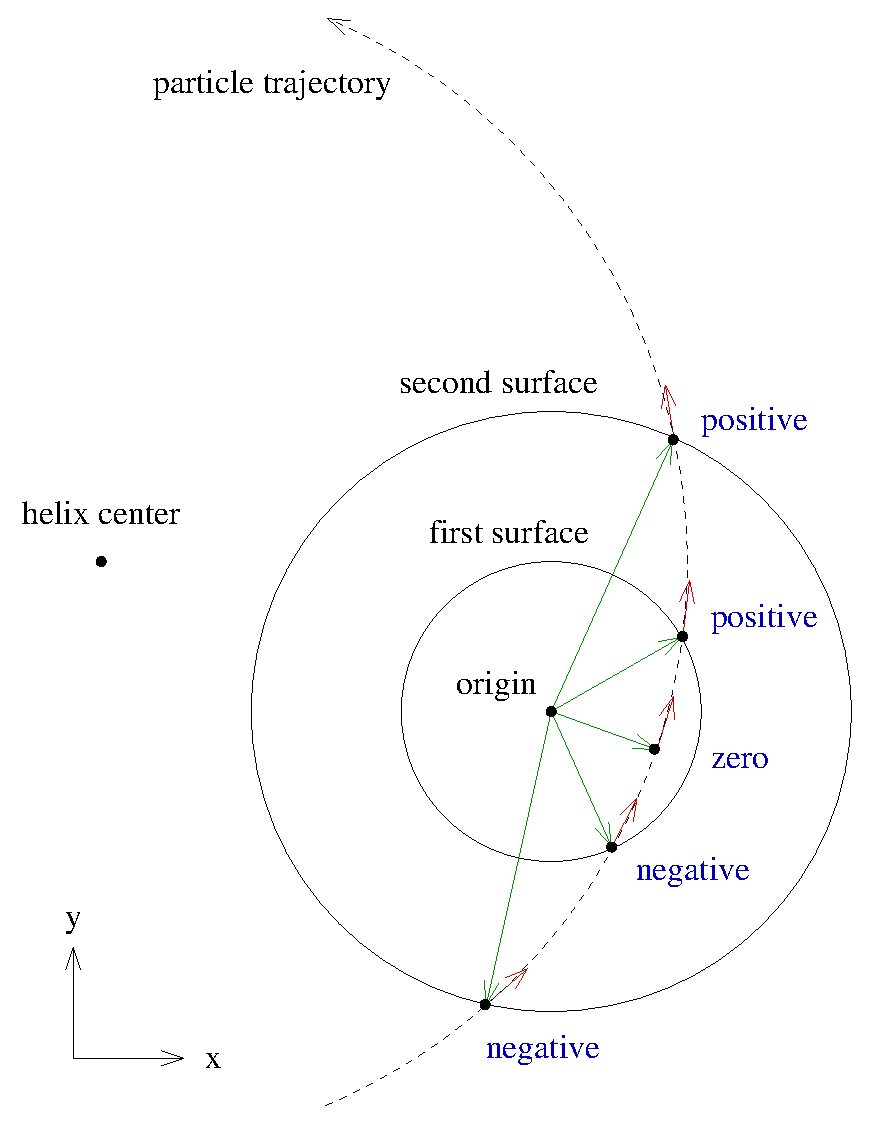
\includegraphics[height=9cm]{xdotp_correct.eps}
\hspace{0.2cm} \begin{minipage}[b]{7cm}
Kalman's algorithm:
\begin{enumerate}

  \item Find a surface intersection in X-Y.

  \item Check that the track's Z \mbox{intersects} the surface.

  \item If not the first surface, be sure that $x p_x + y p_y$ hasn't
  changed sign.

  \item If not, apply scattering and hit if applicable.

\end{enumerate}

\vspace{0.3cm}

\end{minipage}

\vspace{0.5cm}

If the track misses the first surface in Z, Kalman erroneously
compares against the sign of zero, which is unpredictable due to
round-off error.

\vspace{0.5cm}

If $x p_x + y p_y$ at the point of closest approach is $-\epsilon$,
Kalman won't add any hits, leaving the error matrix huge.

\end{minipage}

\end{slide*}

% %%%%%%%%%%%%%%%%%%%%%%%%%%%%%%%%%%%%%%%%%%%%%%%%%%%%%%%%%%%%%%%%%%%%%%%%%%%

\begin{slide*}

\slideframe{}
\slideframe*[\dkblue]{Oval}
\huge
\heading{BigErrorMatrix Bug {\it (continued)}}
\Large

\begin{minipage}[t]{\linewidth}

\vspace{0.2cm}

\begin{itemize}

  \item {\it Inward fits are immune} because the first calculation \\
  of $x p_x + y p_y$ is not at the point of closest approach.

\end{itemize}

\begin{tabular}{l p{0.2cm} r} \hspace{-0.38cm}
  \begin{minipage}[b]{0.62\linewidth}
    \begin{itemize}

      \item About 10\% of outward fits are affected \\
	{\it when the MissingBeamWall bug is also present.}

      \vspace{0.3cm}

      The frequency is platform independent.

      \vspace{0.6cm}

    \end{itemize}
  \end{minipage} & &
  \begin{minipage}[b]{0.3\linewidth}
    \begin{center}
      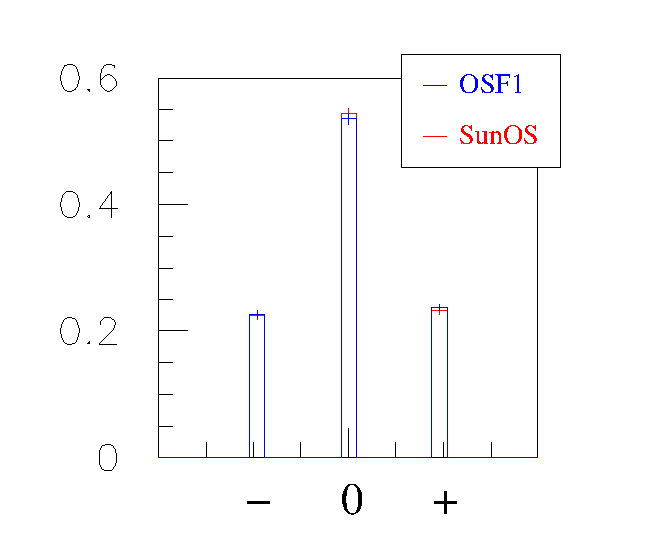
\includegraphics[width=0.95\linewidth]{xdotp_distributions.eps} \\
      Sign of $x p_x + y p_y$
    \end{center}
  \end{minipage} \\
\end{tabular}

\begin{itemize}

  \item Affected outward fits have a large error matrix,
  \begin{itemize}
    \item no RICH information (check {\tt hypWasAnalyzed()}), and
    \item tiny {\tt numberHits()}, {\tt degreesOfFreedom()}
          and {\tt chiSquare()}.

  \vspace{0.3cm}

  \begin{center}\includegraphics[width=\linewidth]{/home/mccann/kalman2/rzn/side-by-side-modified.eps}\end{center}
  \end{itemize}

\end{itemize}

\end{minipage}

\end{slide*}

% %%%%%%%%%%%%%%%%%%%%%%%%%%%%%%%%%%%%%%%%%%%%%%%%%%%%%%%%%%%%%%%%%%%%%%%%%%%

\begin{slide*}

\slideframe{}
\slideframe*[\dkblue]{Oval}
\huge
\heading{Are Data and Monte Carlo the Same?}
\Large

\begin{minipage}[t]{\linewidth}

\vspace{0.5cm}

Unfortunately, no.

\vspace{0.5cm}

\begin{center} \small
\begin{tabular}{l l l}
{\bf Dataset} \hspace{0.5cm} & {\bf Pass2 Release} \hspace{0.5cm} & {\bf Monte Carlo Release} \\\hline
Data8   & {\tt cleo3\_Pass2\_Oct09\_2001} & {\tt cleo3\_MCPS2\_Jan30\_2002} \\
Data15  & {\tt cleo3\_Pass2\_Nov27\_2001} & {\tt cleo3\_MCPS2\_Jan30\_2002} \\
Data7   & {\tt cleo3\_Pass2\_Nov27\_2001} & {\tt cleo3\_MCPS2\_Jan30\_2002} \\
Data16  & {\tt cleo3\_Pass2\_Jan30\_2002} & {\red \tt Jun27\_02\_MC$^*$} \\
Data17  & {\tt cleo3\_Pass2\_Mar26\_2002} & {\red \tt Jun27\_02\_MC$^*$} \\
Data11  & {\tt cleo3\_Pass2\_Mar26\_2002} & {\red \tt Jun27\_02\_MC$^*$} \\
Data5   & {\tt cleo3\_Pass2\_Mar26\_2002} & {\red \tt Jun27\_02\_MC$^*$} \\
Data6   & {\tt cleo3\_Pass2\_Mar26\_2002} & {\red \tt Jun27\_02\_MC$^*$} \\
Data18  & {\red \tt Jul13\_02\_P2$^*$}    & {\red \tt TBA} \\
Data9   & {\red \tt Jul13\_02\_P2$^*$}    & {\red \tt TBA} \\
Data20  & {\red \tt Oct18\_02\_P2$^*$}    & {\red \tt TBA} \\
Data21  & {\red \tt Nov04\_02\_P2$^*$}    & {\red \tt TBA} \\
Data10  & {\tt Nov04\_02\_P2}             & {\tt TBA} \\
\end{tabular}
\end{center}

{\red \small $^*$Releases with the bug.}

\vspace{0.5cm}

Data16, 17, 11, 5, and 6 have the bug in Monte Carlo but not in data.

\end{minipage}

\end{slide*}

% %%%%%%%%%%%%%%%%%%%%%%%%%%%%%%%%%%%%%%%%%%%%%%%%%%%%%%%%%%%%%%%%%%%%%%%%%%%

\begin{slide*}

\slideframe{}
\slideframe*[\dkblue]{Oval}
\huge
\heading{Bug Fixes}
\Large

\begin{minipage}[t]{\linewidth}

\vspace{1cm}

The following bug fixes are part of a patch on {\tt Nov04\_02\_P2}:

\vspace{0.5cm}

\begin{itemize}

\item {\bf MissingBeamWall:} Kalman's internal representation of
beamwall objects has been extended to 100 meters to ensure that no
track can escape the wall in Z.

\vspace{0.5cm}

This fix removes the condition that allowed BigErrorMatrix to be
frequent.

\vspace{1cm}

\item {\bf BigErrorMatrix:} The check of the sign of $x p_x + y p_y$
is now protected by an additional test that it is sufficiently far
from zero ($10^{-10}$).

\vspace{1cm}

\item The RICH code has been updated to look at other candidates or
  inward fits if an error matrix is unreasonably large.

\end{itemize}

\end{minipage}

\end{slide*}

% %%%%%%%%%%%%%%%%%%%%%%%%%%%%%%%%%%%%%%%%%%%%%%%%%%%%%%%%%%%%%%%%%%%%%%%%%%%

\begin{slide*}

\slideframe{}
\slideframe*[\dkblue]{Oval}
\huge
\heading{Summary}
\Large

\begin{minipage}[t]{\linewidth}

\begin{itemize}

  \vspace{0.3cm}

  \item Half the tracks in affected datasets do not scatter in the
  beampipe.  This correction is only as large as 0.1\% for tracks
  under 600 MeV.  It changes error matrix elements by as much as
  $1/5^{\mbox{th}}$.

  \vspace{0.3cm}

  \item 10\% of the tracks in affected datasets are not properly
  outward-fit.  They are easily identifiable by
  \begin{center}{\tt
  track\_iterator->exitPionQuality()->numberHits() < 3}.\end{center}
  Nothing is wrong with their inward fits.  They even have normal
  residual distributions.

  \vspace{0.3cm}

  \item RICH failed on $2/3$ of these tracks because of a large error
  matrix.  For these,
  \begin{center}{\tt
  track\_iterator->richInfo()->pionHypWasAnalyzed()}\end{center}
  has been set to {\tt false}.

  \vspace{0.3cm}

  \item Data16, 17, and 11 (and potentially 5 and 6) Monte Carlo
  samples have the bug, while the data does not.

  \vspace{0.3cm}

  \item Data18, 9, 20 and 21 have the bug in data.

  \vspace{0.3cm}

  \item The patch of the {\tt Nov\_04\_02\_P2} code release will not
  have the bug, nor will subsequent datasets.

\end{itemize}

\end{minipage}

\end{slide*}

% %%%%%%%%%%%%%%%%%%%%%%%%%%%%%%%%%%%%%%%%%%%%%%%%%%%%%%%%%%%%%%%%%%%%%%%%%%%

% \begin{slide*}

% \slideframe{}
% \slideframe*[\dkblue]{Oval}
% \huge
% \heading{}
% \Large

% \begin{minipage}[t]{\linewidth}

% \end{minipage}

% \end{slide*}

\end{document}

% %%%%%%%%%%%%%%%%%%%%%%%%%%%%%%%%%%%%%%%%%%%%%%%%%%%%%%%%%%%%%%%%%%%%%%%%%%%

% \begin{slide*}

% \slideframe{}
% \slideframe*[\dkblue]{Oval}
% \huge
% \heading{}
% \Large

% \begin{minipage}[t]{\linewidth}

% \end{minipage}

% \end{slide*}
